\documentclass[11pt]{ekblite}
\newcommand\mtop{1in}
\newcommand\mbottom{1in}
\newcommand\mleft{1.2in}
\newcommand\mright{1.2in}
\usepackage[top=\mtop, bottom=\mbottom, left=\mleft, right=\mright]{geometry}

\newcommand{\comment}[1]{}
\newcommand\aaron[1]{\textcolor{red}{#1}}
\newcommand{\seay}[1]{\textcolor{blue}{#1}}
\hypersetup{ 	
pdfsubject = {Mathematics},
pdftitle = {Fractal Dimension},
pdfauthor = {Max Seay and Aaron Huntley}
}

\begin{document}

\title{Exploring fractal dimension\\
DRP spring 2025}
\maketitle
\begin{center}
	Max Seay and Aaron Huntley\\
\today
\end{center}

\tableofcontents

\newpage

\section{Preface}
This was written by Max Seay of CWRU with direction from PhD student Aaron Huntley, as part of the Directed Reading Program in Spring 2025. As of writing, it has not been proofread. Date of latest update on cover page.

\newpage
\section{Introduction}
The following notes describe concepts of measurement, dimensionality and fractal objects living within metric spaces. The goal is to understand how to compute the \textit{dimensionality} of arbitrarily defined objects. It's already assumed that common objects attain dimensionality of whole numbers. For example: the point is of dimension 0, the line is of dimension 1, the filled square is of dimension 2, the filled cube is of dimension 3, etc. However these notes also describe how dimensionality can be computed for other, more strangely behaved objects. Objects such as \textit{fractals} can attain more unexpected values of measure and dimensionality. For example: the Cantor Set of the real number line $\R$, which takes on non-integer dimensionality of $\frac{\log 2}{\log 3}$, while also having a length of 0. Or the Dragon Curves: a family of space-filling fractal curves derived from the repition of bending of a line towards infinity, which acheive positive area and have the ability to cover and tile the plane of real numbers, $\R^2$.
\begin{definition}[Object]
	A finite or infinite \textit{compact} set $S$ living within some metric space.
\end{definition}
Below are listed further examples of objects, defined from sets, and their corresponding dimensionality:
\begin{itemize}
	\item $\{0\} \in \R$ \\[0.1in] dimensionality: 0
	\item $\{1\} \in \R$ \\[0.1in] dimensionality: 0
	\item $\{2,4,6,8\} \in \R$ \\[0.1in] dimensionality: 0
	\item $[0,1] \in \R$ \\[0.1in] dimensionality: 1
	\item $(0,1) \in \R$ \\[0.1in] dimensionality: 1
	\item $(0,1] \in \R$ \\[0.1in] dimensionality: 1
	\item  $[0,1] \times [0,1] \in \R^2$ \\[0.1in] dimensionality: 2
\end{itemize}

\newpage
\section{How to measure the real numbers}
\begin{figure}[h]
	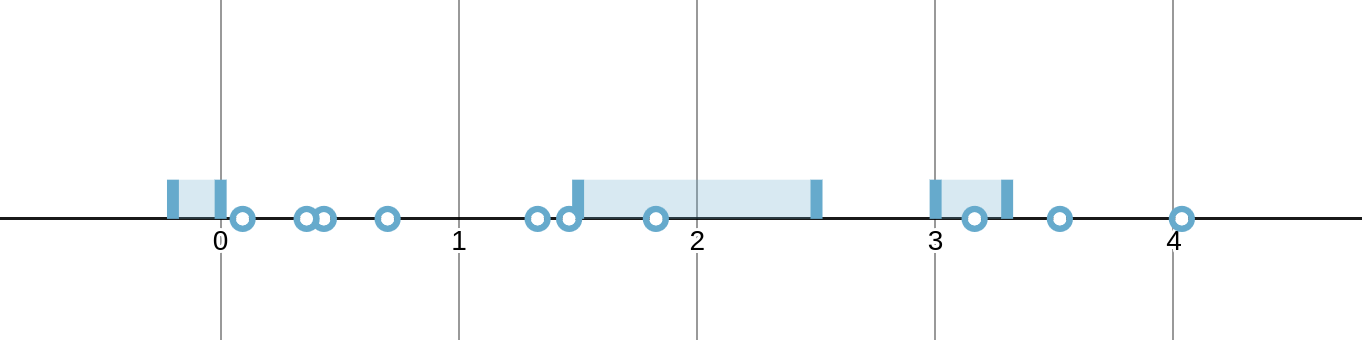
\includegraphics[scale=0.3]{img/c10.jpg}
	\caption{Points and line segments living within the real number line $\R$.}
\end{figure}
On the real number line $\R$, common objects can be defined. For example:
\begin{example}[Point]
	A point on the real number line is a single real number. Examples include: $1,2,3,17,\sqrt{2},\pi$.
	\\[0.2in]The dimensionality of a point is commonly known to be 0. A point can't have length.
\end{example}
\begin{example}[Line segment]
	A line segment on the real number line is the defined to be the set of all real numbers that lie between two points. A line segment that starts at 0 and reaches 1 would be defined as the set
	\[\{x : 0 \le x \le 1\}\] 
	equivalently expressed in \textit{interval form}:
	\[[0,1]\]
	In other words, a set containing every real number between and including 0 and 1.
	\\[0.2in]The dimensionality of a line is commonly known to be 1. 
\end{example}

\begin{definition}[Interval length]
	Given an interval $I$ of the form $[a,b]$, $(a,b)$, $(a,b]$, or $[a,b)$ where $a \le b$, the length of $I$, notated as $|I|$, is defined to be
	\[|I| := b - a\]
\end{definition}
This is intuitive and useful. But how can this be justified with some definition of measure? And how can this idea of length be extended to a more general way of measurement? 
\subsection{Coverings}
Most definitions of measure and dimension involve the idea of a $\textit{covering}$.
\\[0.2in]A $\textit{covering}$ is some collection of sets that cover some other set. If the covering is made from open sets, it's called an open covering.
\begin{example}[Open covering for an interval]
	Let $I = [1,3]$. An example of an open cover for $I$ is
	\[C = \{(-50,0),(-20,70),(50,100)\}\]
	since 
	\[I \subseteq \bigcup C_i\]
	and every set $C_i$ in $C$ is open.
	\\[0.2in]You could say that $C$ is ``overkill'' as an open cover for $I$ since it spans a much longer length than $I$. In this case, the length of the open cover $\bigcup C_i$ is
	\[100 - (-50) = 150\]
	and the length of $I$ is
	\[3 - 1 = 2\]
\end{example}

\subsection{Infinite sequences of sets}

\begin{example}[Stick cutting]
	Let there be some stick $s$ to measure. Say the stick begins at a length of 1. Now do the following:
	\\[0.2in]Cut the stick to $\frac{1}{2}$ its original length. Then take the stick and cut it to $\frac{1}{3}$ its original length. Then cut the stick to $\frac{1}{4}$ its original length. Continue this forever.
	\\[0.2in]At the end of the cutting process, how long is the stick?
	\\[0.2in]Unfortunately this question doesn't make sense. There is no ``end'' to the cutting process since it goes on forever. First the object should be defined in a valid way. Say $s_0$ is the stick before cutting, $s_1$ is the stick at the first cutting step etc.
	\\[0.2in]A valid definition of the object to be measured is:
	\[\bigcap_{i=0}^{\infty} s_i\]
	In other words, the intersection of every stick. The object to be measured is the set of points that are inside each and every stick $s_i$. Now there is no longer any ambiguity.
	\\[0.2in]Another object which represents this length value is the limit
	\[\lim_{i \rightarrow \infty} |s_i|\]
	\\where $s_i$ = $[0,\frac{1}{i+1}]$ represents the stick after step $i$ of the cutting process.	
	\\[0.2in]In other words, the length of each stick in the sequence as the sequence tends towards infinity.
	\\[0.2in]On one hand, the stick is cut forever, so it must be reduced to nothing by the end. On the other hand, the amount that gets cut off decreases each time and so at some point there may be no more cut off at all.
	\\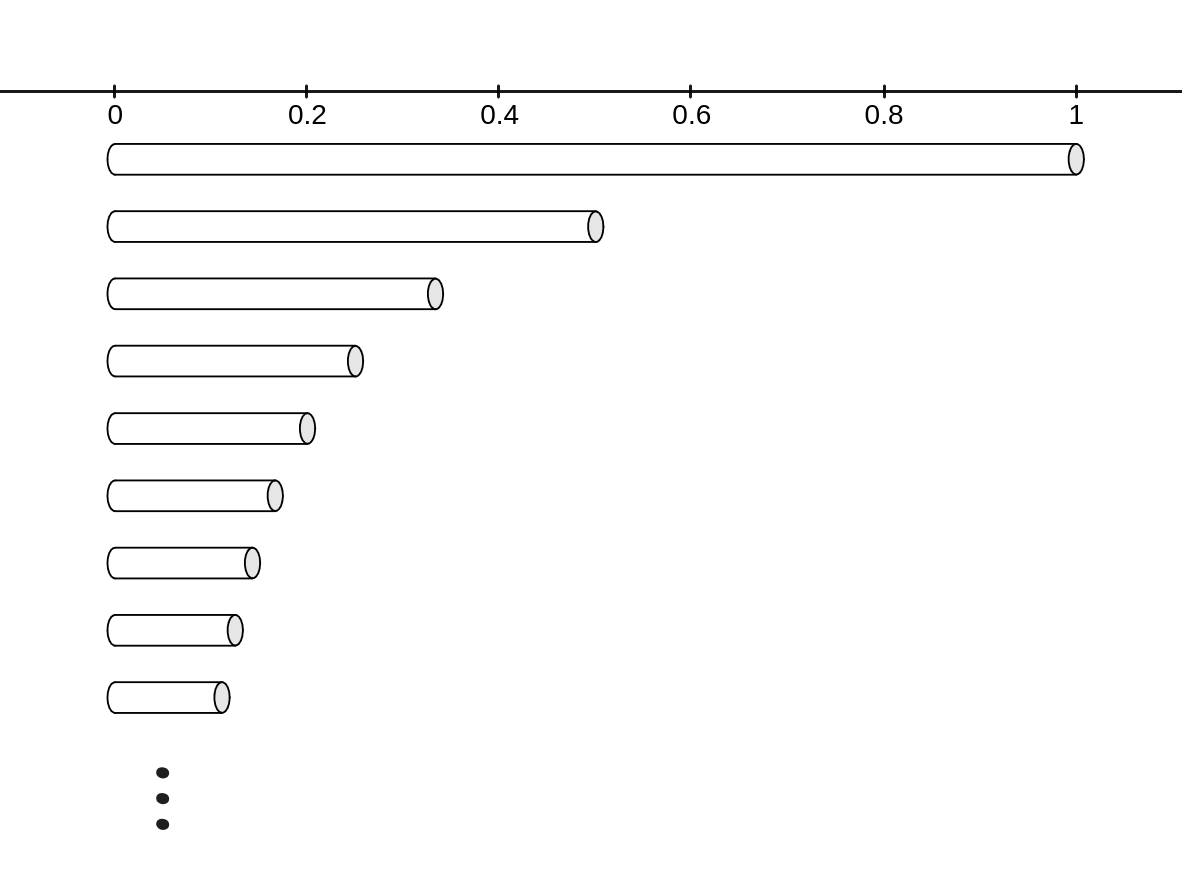
\includegraphics[scale=0.33]{img/c5.jpg}
	\\\textit{Diagram of the first 9 steps of stick cutting.}
	\begin{corollary}
		For each stick $s_i$ in the sequence of sticks $\{s_i\}_{i=1}^{\infty}$, $s_{i} \subset s_{i-1}$. Each stick $s_i$ is covered by stick $s_{i-1}$. 
		\end{corollary}
	\begin{corollary}
	\[\lim_{i \rightarrow \infty} |s_i| = 0\]
	where $s_i$ = $[0,\frac{1}{i+1}]$ represents the stick after step $i$ of the cutting process.	
	\end{corollary}
	\begin{proof}
		Rewrite the limit with the definition of the length of $s_i$: 
		\[\lim_{i \rightarrow \infty} |s_i| = \lim_{i \rightarrow \infty} \left(\frac{1}{i+1} - 0 \right)\]
		So we have
		\[\lim_{i \rightarrow \infty} |s_i| = \lim_{i \rightarrow \infty} \left(\frac{1}{i+1} - 0 \right)= \lim_{i \rightarrow \infty} \left(\frac{1}{i+1} \right)\]
		This is a common limit known to be
		\[\lim_{i \rightarrow \infty} \left(\frac{1}{i+1} \right) = 0\]
		Thus we have that
		\[\lim_{i \rightarrow \infty} |s_i| = 0\]
		as required.
	\end{proof}
	\begin{corollary}
		The length of $\cap_{i=1}^{\infty} s_i$ is 0. 
	\end{corollary}
	To prove this, I will show that given any real number $\varepsilon > 0$, the length of the stick is less than $\varepsilon$. Thus the length must be 0.
	\begin{proof}
		Let the stick be an interval (line segment). Let $s_0$ be the initial stick; a closed interval $[0,1]$.
		\\[0.2in]Step $1$ is to cut the interval in half. So the interval becomes $\left[0,\frac{1}{2}\right]$.
		\\[0.2in]Step $2$ is to cut the interval into a third. So the interval becomes $\left[0,\frac{1}{3}\right]$.
		\\[0.2in]Step $3$ is to cut the interval into a fourth. So the interval becomes $\left[0,\frac{1}{4}\right]$.
		\\[0.2in]Step $k$ is to cut the interval $\left[0,\frac{1}{k}\right]$ into the interval $\left[0,\frac{1}{k+1}\right]$.
		\\[0.2in]After every step of the cutting process, the stick is cut; the length of the interval is decreased. This can be seen by comparing the lengths of the stick before and after some cutting step $k$:
		\[\left| 0 - \frac{1}{k+1} \right| \le \left| 0 - \frac{1}{k} \right|\] 
		\\[0.2in]Let $\varepsilon \in \R^+$ be some arbitrary positive real number.
		\\[0.2in]I will show that there always exists a cutting step $k'$ such that after this step, the length of the stick is less than the arbitrarily small $\varepsilon$. 
		\\[0.2in]Choose the $k'$ step to be a whole number such that
		\[k' > \frac{1}{\varepsilon}\]
		(By the archimedian principle this is always possible.)
		\\[0.2in]I know that by definition of the cutting process, for this step $k'$, the stick is cut to a length $l$ that is
		\[l \le \frac{1}{k'}\] 
		And note that by the definition of $k'$ we have that
		\[l \le \frac{1}{k'} < \frac{1}{\sfrac{1}{\varepsilon}} = \varepsilon\]
		Or simply
		\[l < \epsilon\]
		Since the length of the stick $l$ at some step $k'$ is always less than $\varepsilon$, and $\varepsilon$ can be made arbitrarily small, it must be true that 
		\[l = 0\] 
		As required.
	\end{proof}
\end{example}
\newpage
\begin{figure}[h]
	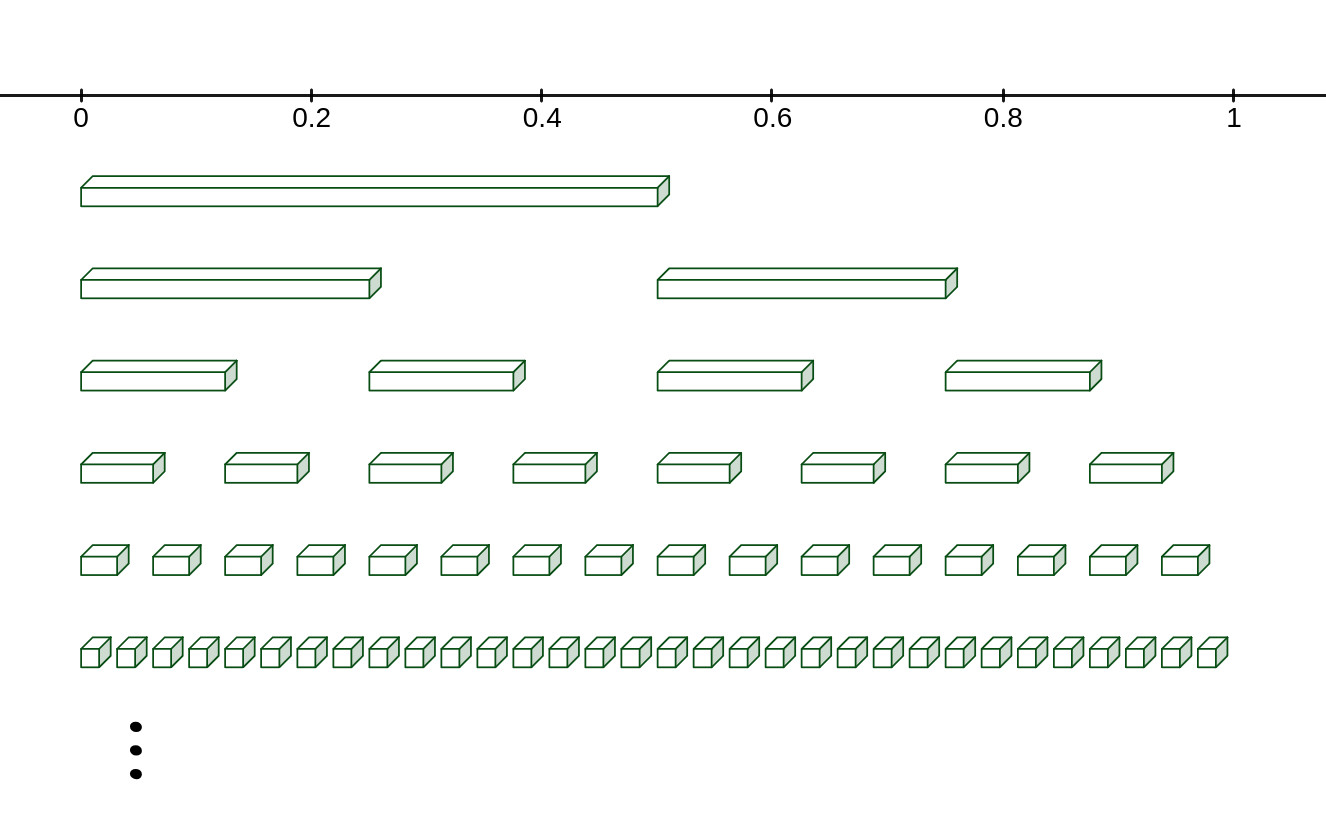
\includegraphics[scale=0.25]{img/c6.jpg}
	\caption{The infinite construction of an object living in the real number line $\R$. On each step, each interval is cut and half and the right half is moved towards the right.}
\end{figure}
\begin{figure}[h]
	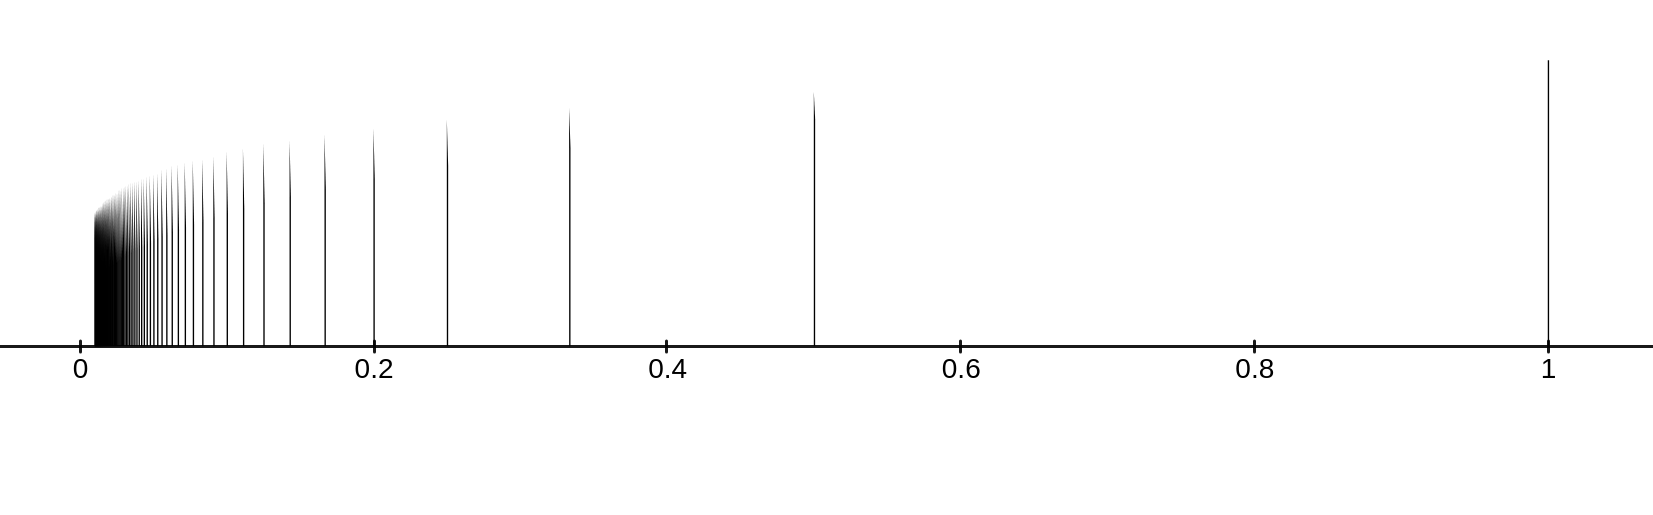
\includegraphics[scale=0.25]{img/c21.jpg}
	\caption{A visual of the sequence $\{\sfrac{1}{n}\}$. A sequence which in fact attains $\sfrac{1}{2}$ dimensionality when considered with box-counting dimension.\cite{japan}}
\end{figure}
A common way of measuring an object is with the construction a covering. When the cover is wrapped around the object, the measure of the cover should be similar to that of the object itself.
\\[0.2in]For example, to measure the surface area of a sphere, a cover could take on the form of a 2-dimensional blanket or sheet, which when tighly wrapped around the sphere covers the entire object. The trivial measurement of the area of the sheet can then be compared to that of the sphere. The idea of covers are often involved with the many varied definitions of measure and dimension.
\subsection{Lebesgue measure}
Lebesgue measure on the real number line is a method of measuring objects within $\R$. The object is nearly wrapped within a collection of intervals, aimed to cover the entire object. As the cover tightens, shrinks or expands, the sum of measurements of the collection approaches that of the object itself.
\\[0.2in]$\textit{Outer}$ Lebesgue measure is to begin with an outside cover that initially overestimates the length of the object, then shrinking it, and approaching the desired measurement.\cite{edgar}
\\[0.2in]$\textit{Inner}$ Lebesgue measure is to begin with an inside cover that underestimates the length of the object, then expanding it, and approaching the desired measurement.\cite{edgar}
\begin{definition}[Lebesgue measure]
	
\end{definition}

\newpage
\section{Notion of dimension: Minkowski–Bouligand or box-counting dimension}
I would like to know how to estimate the dimension of arbitrary objects on the plane $\R^2$. First I will look at simple examples to find out more about the notion of dimension in 2D space.
\begin{example}[Line segment]
	I know what a line segment is. I also know every line segment is 1 dimensional.
	\\[0.2in]I take an approximation. I will cover a line segment with boxes. Each box has diameter (or radius) $r$. (To me it doesn't matter much since the difference between radius and diameter is always just a factor of 2.)
	\\[0.2in]Take the line segment to be the interval $[0,1]$. If $r = 1$, then I need only 1 box to cover the line segment.
	\\[0.2in]If $r = \sfrac{1}{2}$, I will need at least 2 boxes.
	\\[0.2in]If $r = \sfrac{1}{3}$, I will need at least 3 boxes.
	\\[0.2in]If $r = \sfrac{1}{n}$, I will need at least $n$ boxes to cover the line segment.
	\\[0.2in]I will define a function that takes in a radius, $r$, and outputs the least number of boxes of radius $r$ needed to cover the line segment. From the above examples it can be seen that this function is:
	\[\mathcal{N}(r) = \frac{1}{r} \]
	Another idea to think on. How to double the \textit{length} of the line segment? To double the length of the line segment, copy and paste it once, and append the copy onto the end of the original. 
	\\[0.2in]So in other words, to double the length of the line segment, add 1, (or $2^1 - 1$ you could say,) extra copy.
\end{example}
\begin{example}[Square]
	I know what a square is. I also know every square is 2 dimensional.
	\\[0.2in]I take an approximation. I will cover a square with boxes. Each box has diameter (or radius) $r$.
	\\[0.2in]Take the square to be the unit square, $[0,1] \times [0,1]$. If $r = 1$, then I need only 1 box to cover the square. (The box and square are the same.)
	\\[0.2in]If $r = \sfrac{1}{2}$, I will need at least 4 boxes.
	\\[0.2in]If $r = \sfrac{1}{3}$, I will need at least 9 boxes.
	\\[0.2in]If $r = \sfrac{1}{n}$, I will need at least $n^2$ boxes to cover the unit square.
	\\[0.2in]I will define a function that takes in a radius, $r$, and outputs the least number of boxes of radius $r$ needed to cover the square. From the above examples it can be seen that this function is:
	\[\mathcal{N}(r) = \frac{1}{r^2}\]
	Now how to double the \textit{area} of the square? To double the area of the square, copy and paste it three times, and append the copies to three sides of the original. 
	\\[0.2in]So in other words, to double the area of the square, add 3, (or $2^2 - 1$ you could say,) extra copies.
\end{example}
So for the line segment we have that the number of squares of radius $r$ needed to cover it as
\[\mathcal{N}(r) = \frac{1}{r}\]
And for the square we have that the number of squares of radius $r$ needed to cover it as
\[\mathcal{N}(r) = \frac{1}{r^2}\]
From these couple examples it seems that, in general
\[\mathcal{N}(r) = c \left(\frac{1}{r}\right)^d\]
Where $c$ is a constant. It seems that it would be appropriate to call the $d$ in this expression the dimension. This function $\mathcal{N}(r)$ is called a power law since $\sfrac{1}{r}$ is always raised to some power. \cite{falconer2}

\newpage
\section{Notion of dimension: Hausdorff measure and dimension}
\begin{definition}[Diameter of a set]
	Let $S$ be a non-empty set living in $\R^n$. The diameter of $S$ is defined to be 
	\[|S| = \sup \{|x - y| : x,y \in S\}\] 
\end{definition}
\begin{figure}[h]
	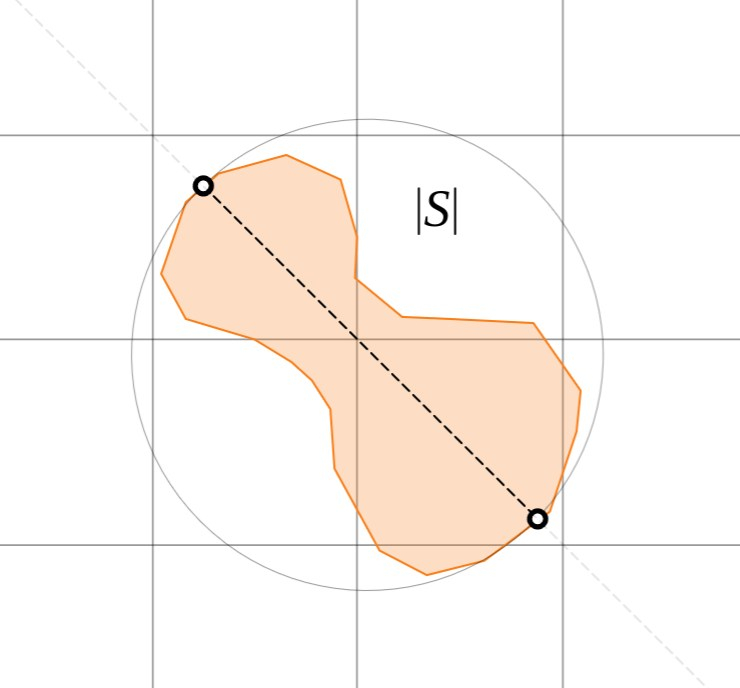
\includegraphics[scale=0.25]{img/c14.jpg}
	\caption{Diameter of a set $S$ living in $\R^2$.}
\end{figure}
\begin{definition}[$\delta$-cover]
	Let $S$ be a set living in $\R^n$. A set of sets $\mathcal{C}$, (where each element $C_i \in \mathcal{C}$ is itself a set), is said to be a $\delta$-\textit{cover} of $S$ if 
	\[S \subseteq \bigcup_{C_i \in \mathcal{C}} C_i\]
	and $|C_i| \le \delta$ for every $C_i \in \mathcal{C}$.\cite{falconer1} 
\end{definition}
\begin{definition}[Hausdorff measure]
	Let $S$ be a set living in $\R^n$. First define the function
	\[\mathcal{H}_{\delta}^{d}(S) = \inf \sum_{i=1}^{\infty} |C_i|^d\]
	where the infimum is taken over each and every possible $\delta$-cover $\mathcal{C}$ of the set $S$.\cite{falconer1}
	\\[0.2in]In other words, this function picks the "tightest" $\delta$-cover of $S$ and sums the diameter of everything in the covering. The "tightest" $\delta$-covering is the $\delta$-covering with the smallest sum.
	\\[0.2in]Define the \textit{Hausdorff measure} of the set $S$ to be the limit:
	\[\lim_{\delta \rightarrow 0} \mathcal{H}_{\delta}^d(S) \]
	And denote this as simply
	\[\mathcal{H}^d(S)\]
\end{definition}
\begin{figure}[h]
	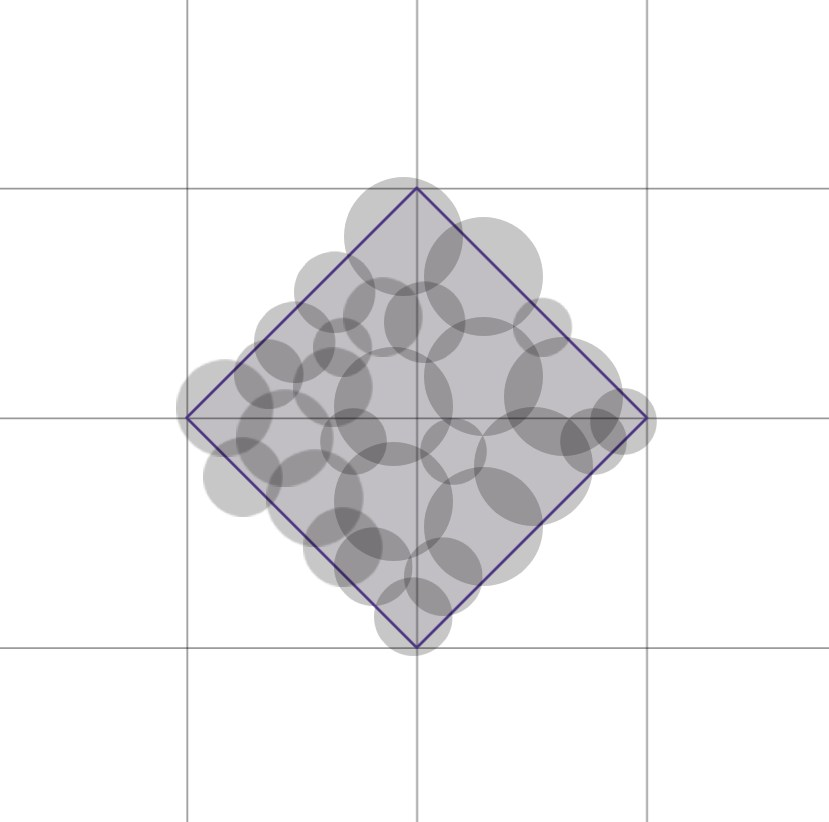
\includegraphics[scale=0.2]{img/c12.jpg}
	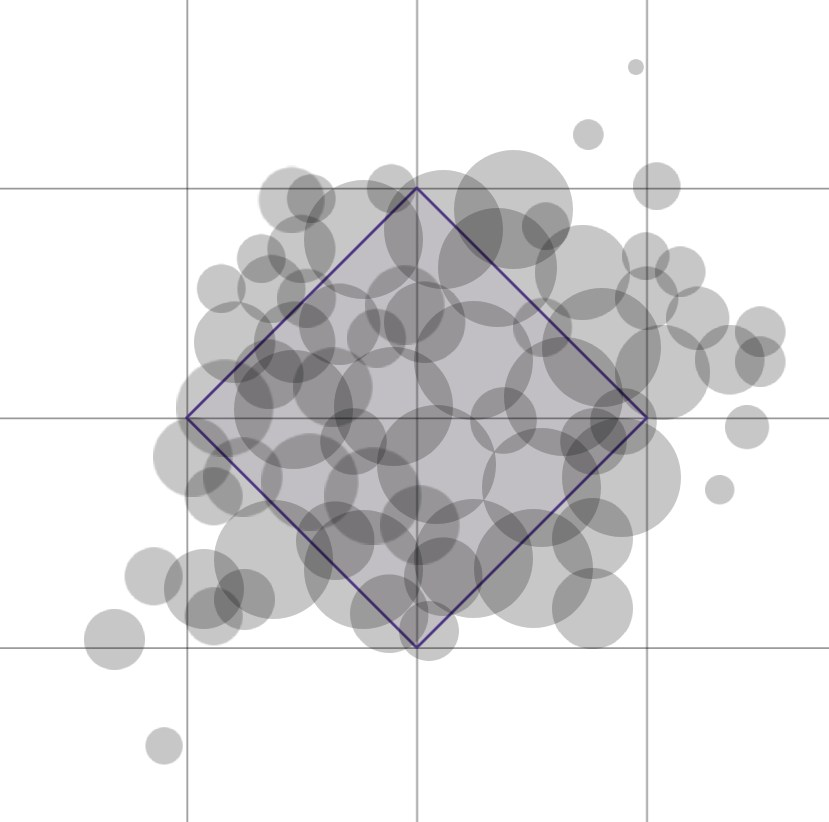
\includegraphics[scale=0.2]{img/c13.jpg}
	\caption{Two valid $\delta$-covers of an object living in $\R^2$. A relatively tight $\delta$-cover (left) compared to a much less tight $\delta$-cover (right). The sum of the diameters of the tight $\delta$-cover (left) is less than the sum of the diameters of the much less tight $\delta$-cover (right). }
\end{figure}
Let's measure some objects using Hausdorff measure.
\begin{example}[Line segment]
	Let $S$ be a line segment living in $\R^2$. Say that
	\[S = [0,1]\]
	The length of $S$ is 1. Though now I would like to compute the measure of this set $S$ using Hausdorff measure. Recall the function
	\[\mathcal{H}_{\delta}^d (S) = \inf \sum_{C_i \in \mathcal{C}} |C_i|^d\]
	where the infimum is taken over every countable $\delta$-cover, $C$, of $S$. Before sending $\delta$ to 0, for now let
	\[\delta = \sfrac{1}{10} \qquad \text{and} \qquad d = 1\]
	With this the function becomes
	\[\mathcal{H}_{\sfrac{1}{10}}^{1} (S) = \inf \sum_{C_i \in \mathcal{C}}^{} |C_i|\]
	where the infimum is taken over each and every possible $\delta$-cover $\{C_i\}$ of $S$ where $\delta = \sfrac{1}{10}$.
	\begin{figure}[h]
		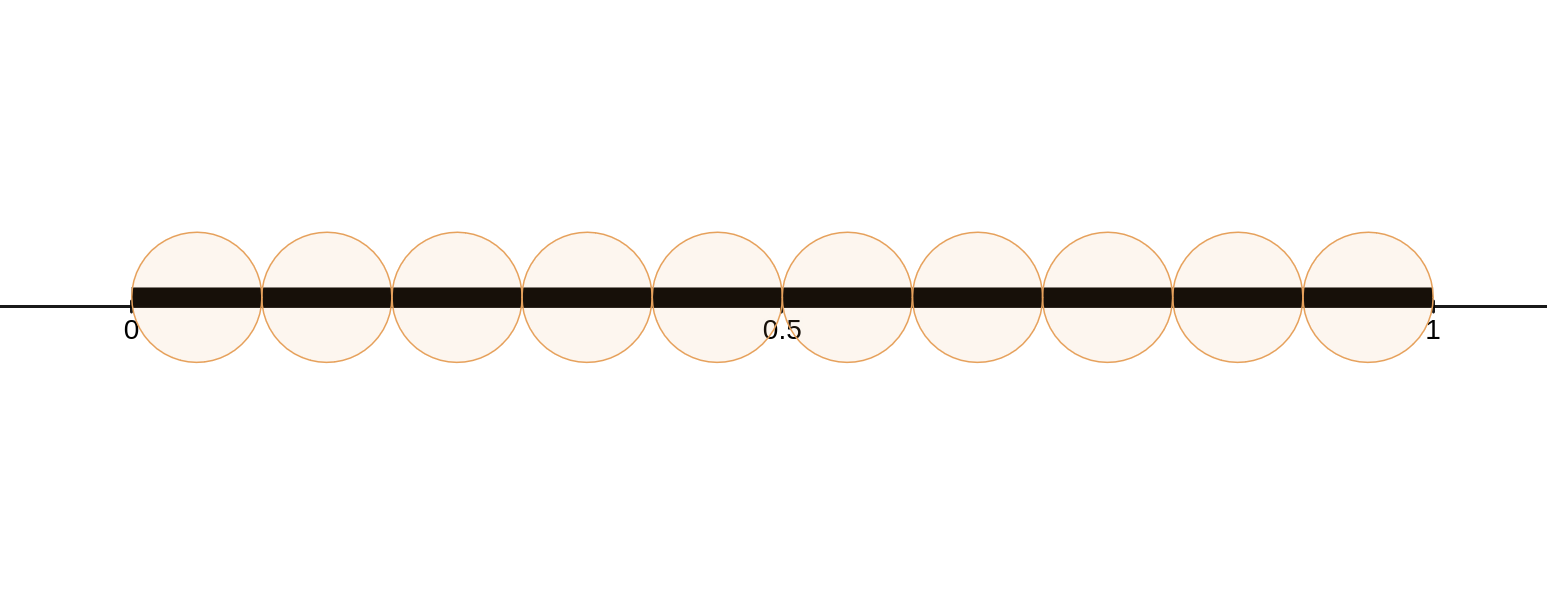
\includegraphics[scale=0.25]{img/c19.jpg}
		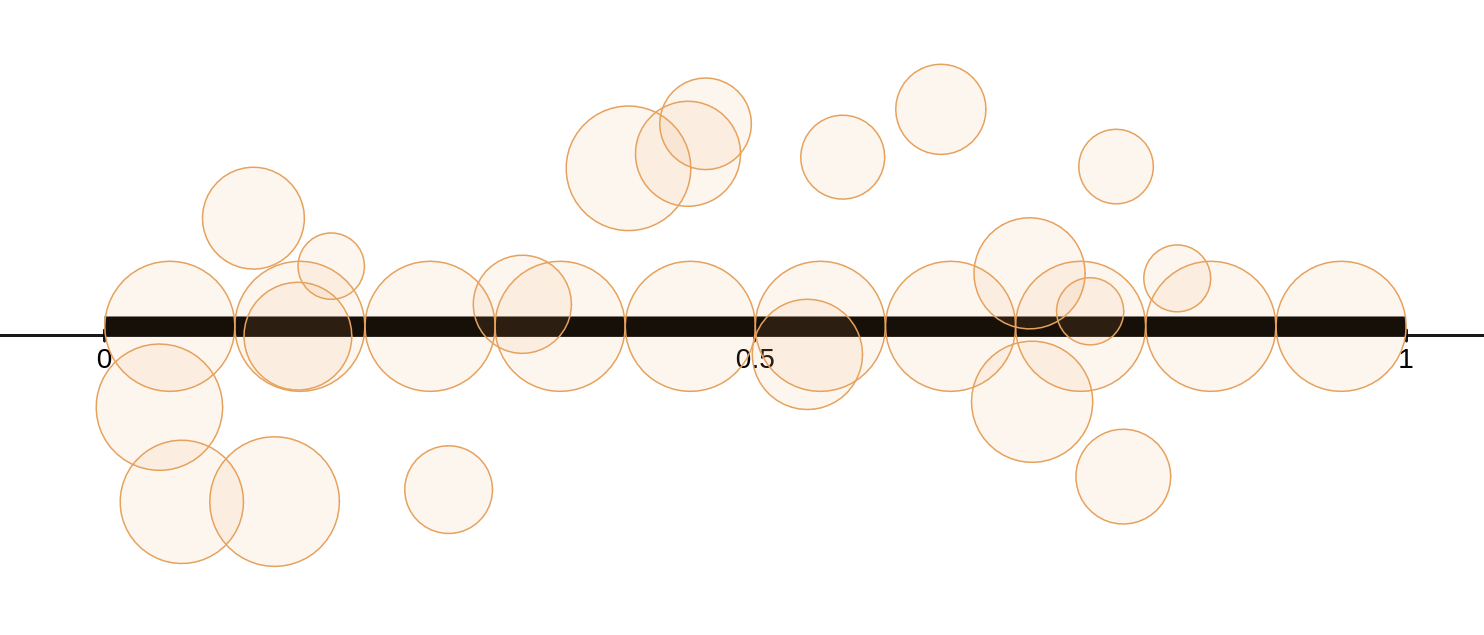
\includegraphics[scale=0.26]{img/c18.jpg}
		\caption{Two ways to cover the line segment [0,1] with a $\delta$-cover where $\delta = \sfrac{1}{10}$. Each orange circle represents an element $C_i \in \mathcal{C}$ of the $\delta$-covering. Notice $[0,1] \subseteq \bigcup_{C_i \in \mathcal{C}} C_i$ and $|C_i| \le \sfrac{1}{10}$ for all $C_i$ (as required of a $\delta$-cover.) Let the top image show the cover $\mathcal{C}$ and the bottom image show the cover $\mathcal{D}$. It can be seen that}
		\[\sum |C_i| < \sum |D_i|\]
		(Roughly speaking because there are less balls in the top cover $\mathcal{C}$ than the bottom cover $\mathcal{D}$.) 
		\label{fig:figure5}
	\end{figure}
	\\[0.2in]Before continuing, make the following assumption:
	\\[0.2in]The infimum covering that the Hausdorff measure uses is to be a cover like that of \ref{fig:figure5} (top image.) That is, the cover is to be arranged such that there are 10 closed balls each with size $\sfrac{1}{10}$ covering the line segment side-by-side. I choose this specific cover \textit{without} proving it is indeed the cover with the infimum sum of diameters, simply because this leads to the expected answer for the measure of $S$.
	\\[0.2in]For each ball in the cover
	\[|C_i| = \sfrac{1}{10}\]
	So we have
	\[\mathcal{H}_{\sfrac{1}{10}}^{1} (S) = \sum_{C_i \in \mathcal{C}} |C_i| = \sum_{C_i \in \mathcal{C}} \sfrac{1}{10} = \left( \frac{1}{10} + \frac{1}{10} + \dots \right) = 1\]
	So this ``approximatation'' of Hausdorff measure, where $\delta = \sfrac{1}{10}$, agrees with intuitition.
	\\[0.2in]Ok now try $\delta = \sfrac{1}{20}$ and consider the same configuration of balls for the $\delta$-cover of $S$. That is, arrange 20 balls side-by-side all of diameter $\sfrac{1}{20}$. Now we have that
	\[\mathcal{H}_{\sfrac{1}{20}}^{1} (S) = \sum_{C_i \in \mathcal{C}} |C_i| = \sum_{C_i \in \mathcal{C}} \sfrac{1}{20} = \left( \frac{1}{20} + \frac{1}{20} + \dots \right) = 1\]
	So this ``approximatation'' of Hausdorff measure, where $\delta$ is even smaller, still agrees with intuitition.
	Now using the same kind of covers as before, send $\delta$ to 0.
	\\[0.2in]And with this the Hausdorff measure can be expressed as
	\[\mathcal{H}^{1} (S) := \lim_{\delta \rightarrow 0} \mathcal{H}_{\delta}^{1} (S)\]
	\[= \lim_{\delta \rightarrow 0} \sum_{C_i \in \mathcal{C}} \delta = \lim_{\delta \rightarrow 0} 1 = 1\]
\end{example}
Note that throughout the above compution of dimensionality, $d=1$ was given. To experiment with this $d$ value, the same conputation can be repeated but instead with a different value of $d$.
\begin{example}[Line segment with $d = 2$]
	Let $S$ be a line segment living in $\R^2$. Say that
	\[S = [0,1]\]
	Again the length of $S$ is 1. Beginning once again with the computation, but now in this case set
	\[\delta = \sfrac{1}{10} \qquad \text{and} \qquad d = 2\]
	With these values we now have the function
	\[\mathcal{H}_{\sfrac{1}{10}}^{2} (S) = \inf \sum_{C_i \in \mathcal{C}} |C_i|^2\]
	where the infimum is taken over every possible $\delta$-cover $\mathcal{C}$ of $S$ where $\delta = \sfrac{1}{10}$. And also now $d=2$.
	\\[0.2in]Again we apply the previous covering, (again assuming it is the correct covering to use), that is, arrangement of balls such that every ball, each with size $\sfrac{1}{10}$, covers the line segment side-by-side.
	\[\mathcal{H}_{\sfrac{1}{10}}^{2} (S) = \sum_{C_i \in \mathcal{C}} |C_i|^2 = \sum \left( \sfrac{1}{10} \right)^2 = \left( \frac{1}{100} + \frac{1}{100} + \dots \right) = \frac{10}{100} = \frac{1}{10}\]
	Note that compared to the Hausdorff measurements of the first example (where $d = 1$) this is smaller.
	\\[0.2in]Ok now try $\delta = \sfrac{1}{20}$ and consider the same configuration of balls for the $\delta$-cover of $S$. That is, arrange 20 balls side-by-side all of diameter $\sfrac{1}{20}$. Now we have that
	\[\mathcal{H}_{\sfrac{1}{20}}^{2} (S) = \sum_{C_i \in \mathcal{C}} |C_i|^2 = \sum \left( \sfrac{1}{20} \right)^2 = \left( \frac{1}{400} + \frac{1}{400} + \dots \right) = \frac{20}{400} = \frac{1}{20}\]
	Again this measurement computes to an even smaller value.
	And now to send $\delta$ to 0. And so we obtain
	\[\lim_{\delta \rightarrow 0} \mathcal{H}_{\delta}^{2} (S) = \lim_{\delta \rightarrow 0} \sum_{C_i \in \mathcal{C}} |C_i|^2 = \lim_{\delta \rightarrow 0} \sum \delta^2 =  \lim_{\delta \rightarrow 0} 0 = 0\]
	Thus we have that the Hausdorff measure when $d = 2$ of the set $S$ where $S = [0,1]$ is
	\[\lim_{\delta \rightarrow 0} \mathcal{H}_{\delta}^{2} (S) = 0\]
	Well by increasing $d$ to 2, the computation has now yeilded an answer which disagrees with intuition.
\end{example}
\begin{example}[Line segment with generalized $d$]
	Now let $d \in \mathbb{R}^+$, that is, let $d$ be any positive real number. With these we compute the Hausdorff dimension by sending $\delta$ to 0.
	\[\lim_{\delta \rightarrow 0} \mathcal{H}_{\delta}^{d} (S) = \lim_{\delta \rightarrow 0} \sum_{C_i \in \mathcal{C}} |C_i|^d = \lim_{\delta \rightarrow 0} \sum \delta^d\]
	And now to analyze this expression for different values of $d$. 
	\\[0.2in]Well as shown above, we have computed that if
	\[d = 1\]
	then
	\[\lim_{\delta \rightarrow 0} \sum_{C_i \in \mathcal{C}} \delta^d = \lim_{\delta \rightarrow 0} \sum_{C_i \in \mathcal{C}} \delta^1 = 1\]
	and also if
	\[d = 2\]
	then
	\[\lim_{\delta \rightarrow 0} \sum_{C_i \in \mathcal{C}} \delta^d = \lim_{\delta \rightarrow 0} \sum_{C_i \in \mathcal{C}} \delta^2 = 0\]
	In fact it can be seen that
	\[d > 1 \implies \lim_{\delta \rightarrow 0} \sum_{C_i \in \mathcal{C}} \delta^d = 0\]
	\[d < 1 \implies \lim_{\delta \rightarrow 0} \sum_{C_i \in \mathcal{C}} \delta^d = \infty\]
	And finally
	\[d = 1 \implies \lim_{\delta \rightarrow 0} \sum_{C_i \in \mathcal{C}} \delta^d = 1\]
\end{example}
\begin{figure}[h]
	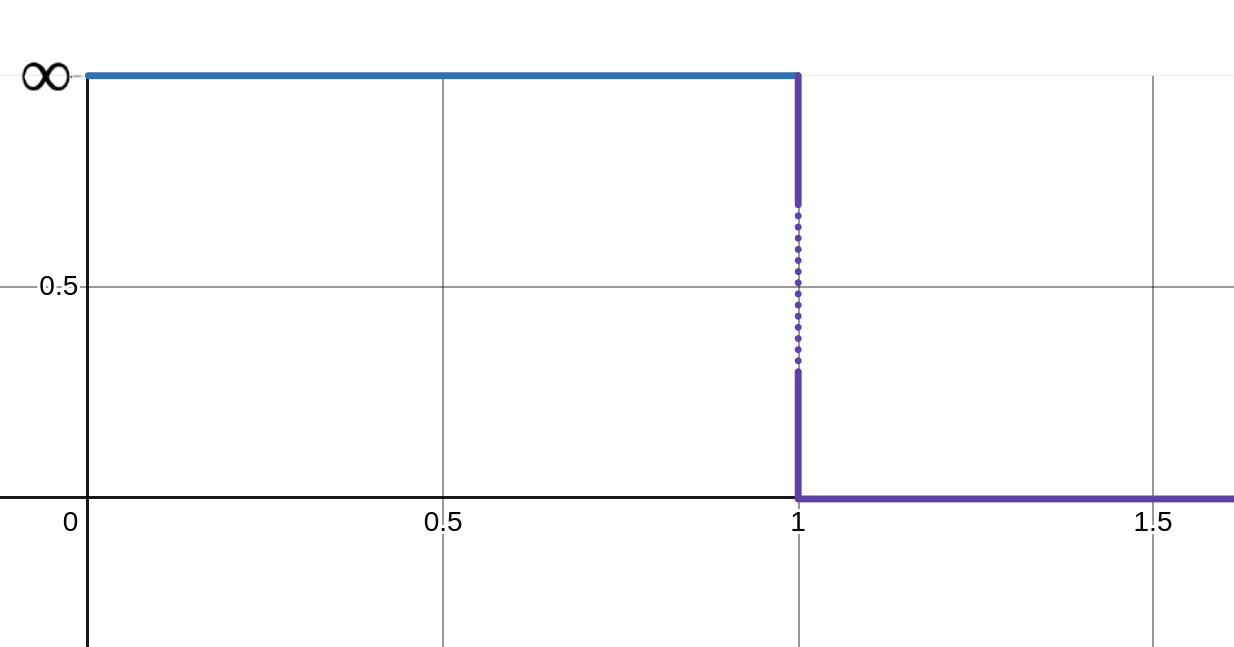
\includegraphics[scale=0.28]{img/c23.jpg}
	\caption{Plot of $d$ vs. $\mathcal{H}^d (S)$}
\end{figure}
\begin{definition}[Hausdorff Dimension]
	In summary, the Hausdorff measure function $\mathcal{H}^d (S)$ as a function with respect to $d$ is a step function. To the left of some \textit{critical value}, $\mathcal{H}^d (S) = 0$ and to the right, $\mathcal{H}^d (S) = \infty$.
	\\[0.2in]And so this critical value is denoted as the \textit{Hausdorff dimension} of a given object. And when the Hausdorff measure $\mathcal{H}^d (S)$ is computed with this critical value, it returns a accurate measurement of the object. To the left, it returns $\infty$. To the right, it returns 0.
\end{definition}

\subsection{Essential properties of the s-dimentional Hausdorff-outer measure}
\begin{corollary}
	$\mathcal{H}^d(\emptyset) = 0$, where $\emptyset$ is the empty set.
\end{corollary}

\begin{corollary}
	Let $X,Y \in \R^n$ such that $X \subset Y$, then
	\[\mathcal{H}^d (X) \le\mathcal{H}^d (Y)\]
\end{corollary}

\begin{corollary}
	Let $\{X_i\}$ be a collection of sets, then
	\[\mathcal{H}^d \left( \bigcup_{i=0}^{\infty} X_i \right) \le \sum_{i=0}^{\infty} \mathcal{H}^d (X_i)\]
\end{corollary}

\begin{corollary}
	Let $\{X_i\}$ be a collection of sets where $X_i$ is a borel set for all $i$, then
	\[\mathcal{H}^d \left( \bigcup_{i=0}^{\infty} X_i \right) = \sum_{i=0}^{\infty} \mathcal{H}^d (X_i)\]
	The category of \textit{borel} sets is massive. Most if not all sets one could think of are borel. All sets (objects) considered in these notes are Borel. Thus a definition isn't needed.
\end{corollary}


\newpage
\section{Cantor Set}
	\begin{figure}[h]
		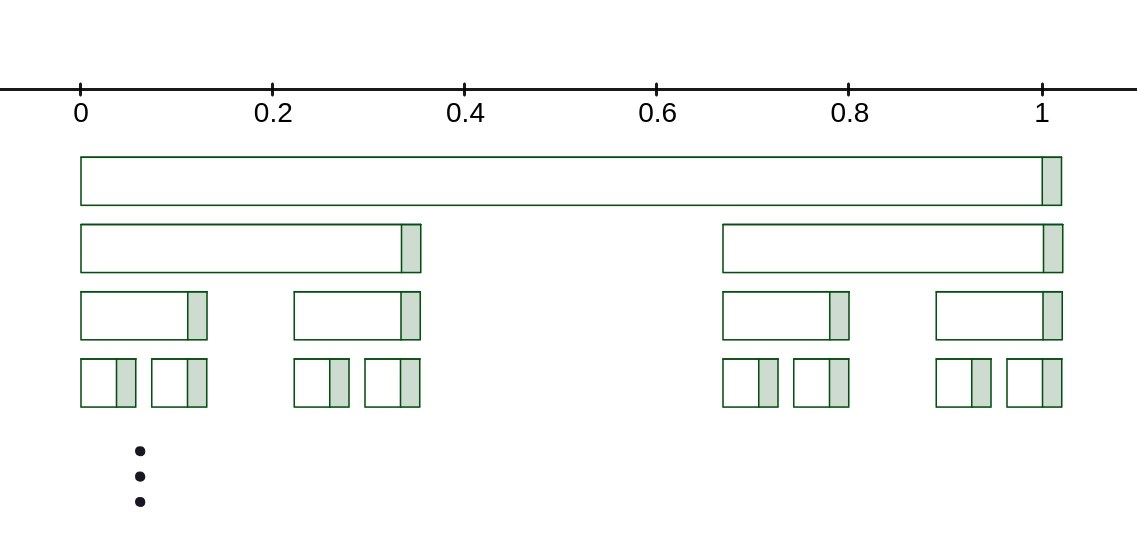
\includegraphics[scale=0.3]{img/c20.jpg}
		\caption{The infinite construction of the Cantor Set in $\R$. On each step, the middle third of each interval is deleted.}
	\end{figure}
	Let $\mathcal{C}$ be the Cantor Set.
	\begin{definition}[Cantor Set]
        $\mathcal{C}$ can be described as an intersection of an infinite sequence of sets. The sequence of sets, $\{\mathcal{C}_i\}_{i=0}^{\infty}$, is defined recursively. For example, the first three are:
		\[C_0 = [0,1]\]
		\[C_1 = \left[0,\sfrac{1}{3}  \right] \cup \left[ \sfrac{2}{3},1\right]\]
		\[C_2 = \left[0,\sfrac{1}{9}  \right] \cup \left[ \sfrac{2}{9},\sfrac{3}{9} \right] \cup \left[\sfrac{6}{9},\sfrac{7}{9}\right] \cup \left[ \sfrac{8}{9},1\right]\]
		\[C_3 = \left[0,\sfrac{1}{27}  \right] \cup \left[\sfrac{2}{27},\sfrac{3}{27}  \right] \cup \left[\sfrac{6}{27},\sfrac{7}{27}  \right] \cup \left[\sfrac{8}{27},\sfrac{9}{27}  \right] \cup \left[\sfrac{18}{27},\sfrac{19}{27}  \right] \cup \left[\sfrac{20}{27},\sfrac{21}{27}  \right] \cup \left[\sfrac{24}{27},\sfrac{25}{27}  \right] \cup \left[\sfrac{26}{27},1  \right]\]
		\\
		And the recursive definition for a set $\mathcal{C}_i$ is:
		\[\mathcal{C}_i = \frac{1}{3}  \mathcal{C}_{i-1} \cup \frac{2}{3} + \frac{1}{3} \mathcal{C}_{i-1}\]
	\end{definition}
	\begin{corollary}
		$\mathcal{C}_i \ne \mathcal{C}$ for all $i \in \mathbb{N}$. No set in the sequence $\{\mathcal{C}_i\}$ is the Cantor Set, however the further you go (the larger the $i$), the ``closer'' $\mathcal{C}_i$ becomes $\mathcal{C}$. 
	\end{corollary}
	\begin{corollary}
		The Cantor Set is non-empty.
	\end{corollary}
	\begin{proof}Consider the point 0.
	\\[0.2in]$0 \in [0,1]$ so $0 \in \mathcal{C}_0$.
	\\[0.2in]Now make the assumption that $0 \in \mathcal{C}_k$.
	\\[0.2in]And since $\frac{1}{3} \cdot 0 = 0$ it must be true that
	\[0 \in \frac{1}{3} \cdot \mathcal{C}_k\] 
	\\[0.2in]Note that by definition we have that
	\[\mathcal{C}_{k+1} = \frac{1}{3} \mathcal{C}_{k} \cup \frac{2}{3} + \frac{1}{3} \mathcal{C}_{k}\]
	Well since $0 \in \frac{1}{3} \cdot \mathcal{C}_k$ it must be true that
	\[0 \in \frac{1}{3} \mathcal{C}_{k} \cup \frac{2}{3} + \frac{1}{3} \mathcal{C}_{k}\]
	or
	\[0 \in \mathcal{C}_{k+1}\]
	So by induction we have that
	\[0 \in \mathcal{C}\]
	Thus $\mathcal{C}$ is non-empty.
	\end{proof}
	\begin{corollary}
		$\mathcal{C}_{i}$ is always a covering of $\mathcal{C}_{i+1}$ and also always a covering of $\mathcal{C}$.
	\end{corollary}
	\begin{corollary}
		There Cantor Set has an infinite number of elements.
	\end{corollary}
	\begin{proof}
		To show the Cantor Set has an infinite number of elements, it suffices to define an injective map between the natural numbers $\N$ and some (or all) elements of the Cantor Set $\mathcal{C}$, thus verifying the cardinality of $\mathcal{C}$ matches or excedes countably infinite number of elements within $\N$.
	\end{proof}
	\newpage
	\begin{figure}[h]
		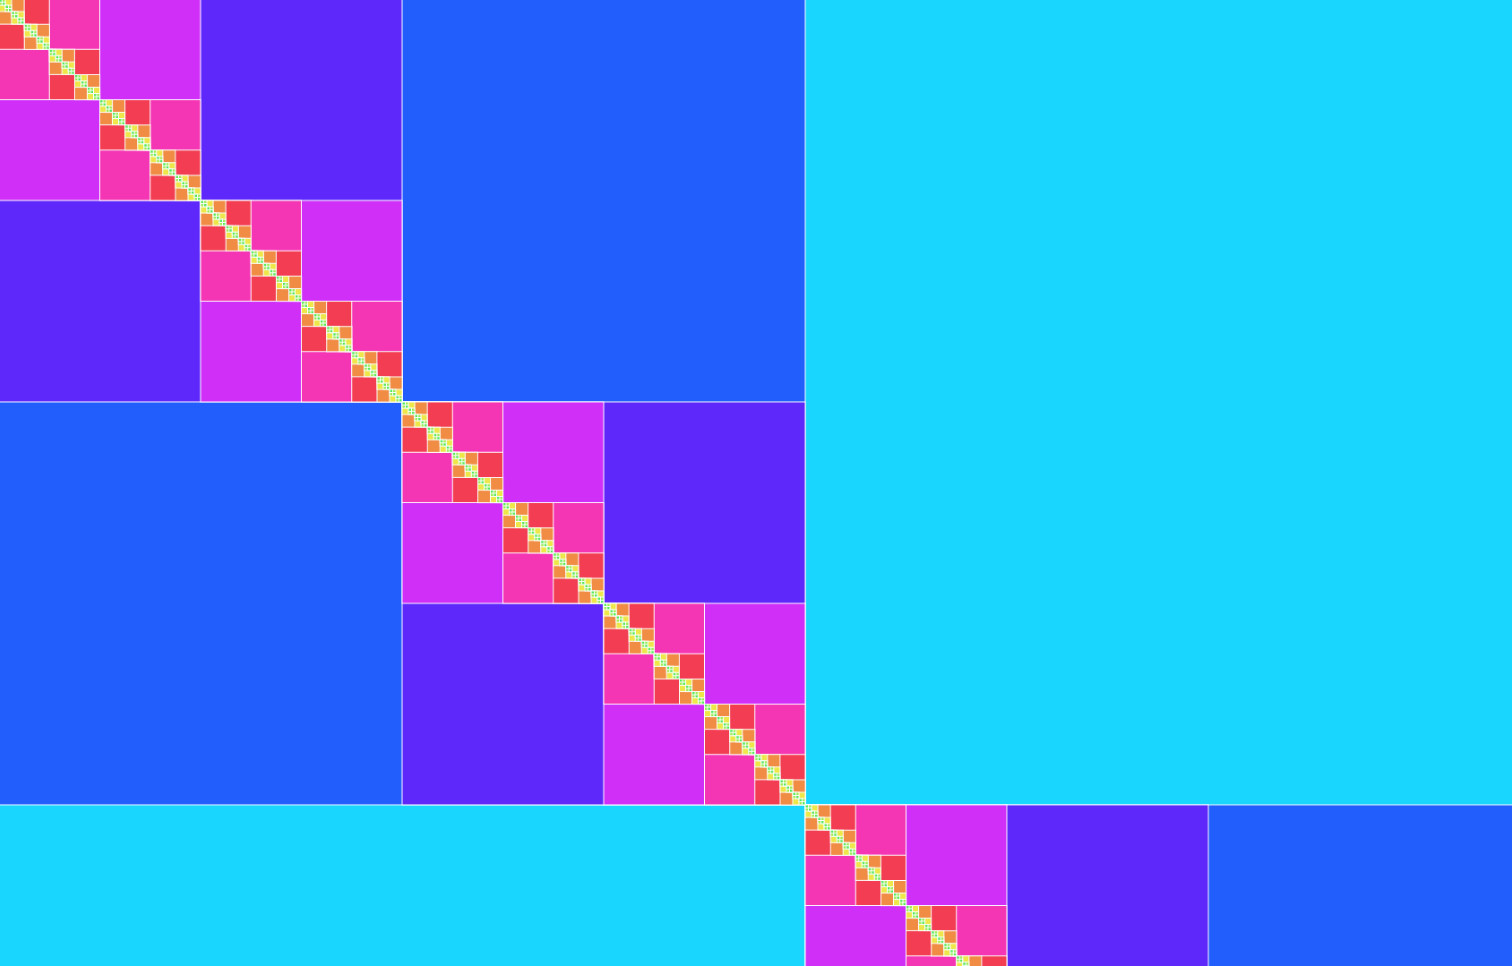
\includegraphics[scale=0.2]{img/c8.jpg}
		\caption{A set visualized in 2D with 10 iterations constructed the same way as the Cantor Set. However the $\frac{1}{3}$ in the Cantor Set definition is replaced with $\frac{1}{2}$ instead.}
	\end{figure}
	\begin{figure}[h]
		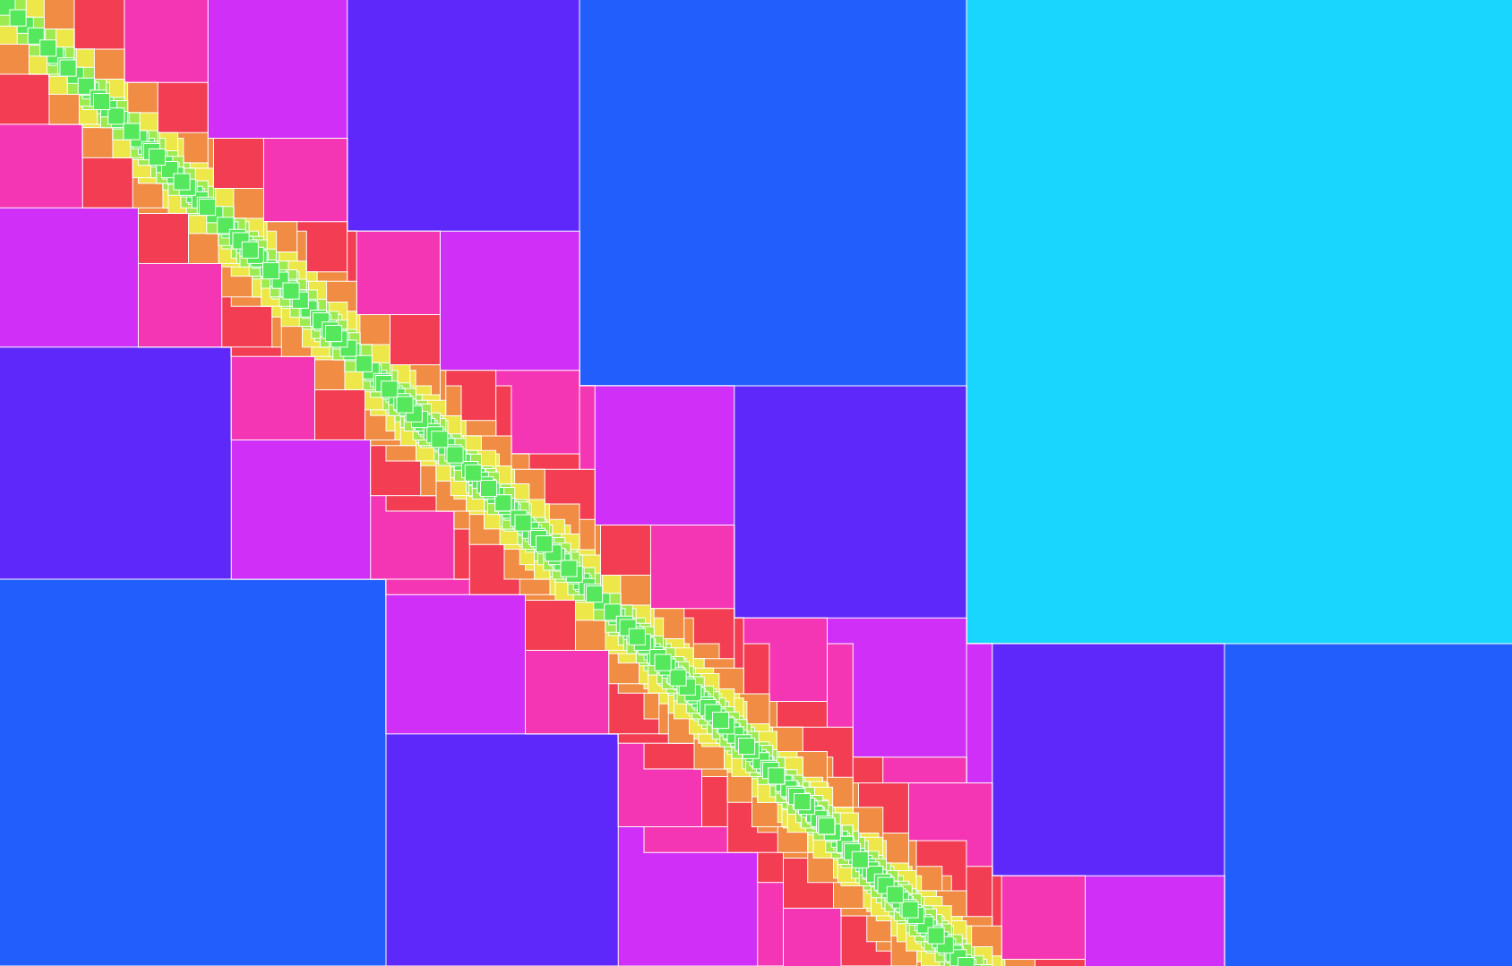
\includegraphics[scale=0.2]{img/c7.jpg}
		\caption{A set visualized in 2D with 10 iterations constructed the same way as the Cantor Set. However the $\frac{1}{3}$ in the Cantor Set definition is replaced with $\frac{3}{4}$ instead.}
	\end{figure}
	\begin{figure}[h]
		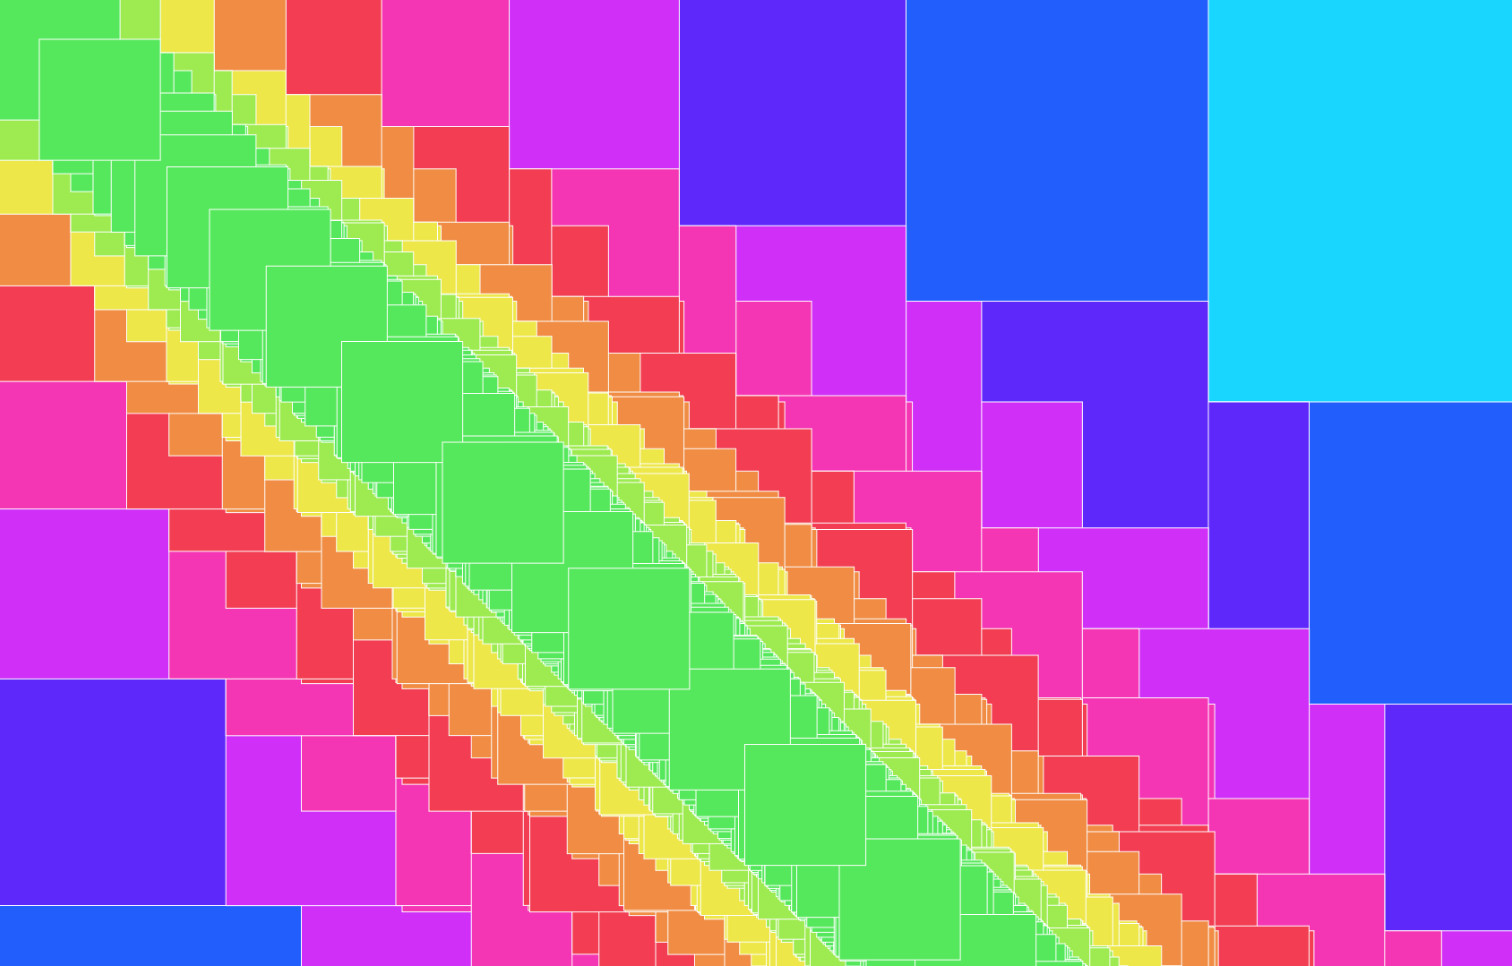
\includegraphics[scale=0.2]{img/c9.jpg}
		\caption{A set visualized in 2D with 10 iterations constructed the same way as the Cantor Set. However the $\frac{1}{3}$ in the Cantor Set definition is replaced with $\frac{4}{5}$ instead.}
	\end{figure}
\newpage
\section{Dragons}

\newpage
\bibliography{citations}

\end{document}
